% Desenvolvido por: Prof. Dr. David Buzatto
%
% Versão 1.6.2
% Data: 21/12/2022

\documentclass[
12pt,
oneside,
a4paper,
chapter=TITLE,
english,
french,
spanish,
brazil,
]{abntex2}

\usepackage{estrutura}
\usepackage[brazilian,hyperpageref]{backref}
\usepackage[alf,abnt-emphasize=bf]{abntex2cite}

% ---
% Dados do documento
% ---

\tipotrabalho{Relatório Técnico}


\titulo{Segmentação de imagens de média e baixa resolução por meio do modelo Segment Anything}
% caso não haja, comente a linha abaixo
%\subtitulo{subtítulo (se houver)}

\autor{Vitor Hugo Fazoli da Silva}
\orientador{Prof. Dr. Gabriel Marcelino Alves}

\curso{Bacharelado em Ciência da Computação}
\grau{Bacharel em Ciência da Computação}

%exemplos
%\curso{Bacharelado em Ciência da Computação}
%\grau{Bacharel em Ciência da Computação em Sistemas para Internet}
%\curso{Especialização em Desenvolvimento de Aplicações para Dispositivos Móveis}
%\grau{Especialista em Desenvolvimento de Aplicações para Dispositivos Móveis}

\campus{São João da Boa Vista}
\area{Computação Gráfica}

\local{São João da Boa Vista}
\mes{MÊS}
\ano{2024}

\instituicao{%
	Instituto Federal de Educação, Ciência e Tecnologia de São Paulo
	\par
	Câmpus \imprimircampus
}

\preambulo{\imprimirtipotrabalho\ Relatório Ténico elaborado conforme a ABNT NBR 10719:10, apresentado ao Instituto Federal de Educação, Ciência e Tecnologia de São Paulo, como parte dos requisitos para a obtenção do grau de \imprimirgrau.
	\\
	\\
	Área de Concentração: Visão Computacional\imprimirarea}

\setlength{\parindent}{1.3cm}
\setlength{\parskip}{0.2cm}

\makeindex

% ---------------------------------------------------------------------------------
%                                   INÍCIO DO DOCUMENTO
% ---------------------------------------------------------------------------------
\begin{document}
	
	% Seleciona o idioma do documento
	\selectlanguage{brazil}
	
	% Retira espaço extra obsoleto entre as frases.
	\frenchspacing 
	
	\pretextual
	\begin{center}
   	
   	\ABNTEXchapterfont\Large\textsc{\imprimirautor}
   	\vspace{2.5cm}
   	
   	\ABNTEXchapterfont\LARGE\textsc{\imprimirtitulo\ifdef{\osubtitulo}{:}{}}

    \ifdef{\osubtitulo}{\ABNTEXchapterfont\Large\imprimirsubtitulo}{}
   	\vspace{2.5cm}
   	   	
   	\hspace{.4\textwidth}
   	\begin{minipage}{.5\textwidth}
   		\SingleSpacing
   		\large\imprimirpreambulo
   		
   		\vspace{\onelineskip}
   		
   		Orientador: Prof Dr.Gabriel Marcelino Alves
        
        
   		
   	\end{minipage}%
    \vfill
   	
   	\Large\textsc{\imprimirlocal}
   	
   	\Large\textsc{2023}
   	
   	\vspace*{2cm}
   	
\end{center}
	\input{02FolhaDeRosto}
	
	% ---
	% Inserir a ficha catalográfica
	% ---
	\input{03FichaCatalografica}
	
	% ---
	% Inserir ata de defesa
	% ---
	\input{04AtaDefesa}
	
	% ---
	% inserir o sumário
	% ---
	\pdfbookmark[0]{\contentsname}{toc}
	\tableofcontents*
	\cleardoublepage
	% ---
	
	\chapter*{}
\noindent{\textbf{RESUMO}}

\noindent{A iluminação é de grande importância para pinturas e esboços digitais nos dias de hoje, pois fornece a percepção de volume ao ambiente. Porém, a iluminação ainda é difícil de replicar em uma imagem digital, pois representa algo muito diferente de um ambiente tridimensional, ainda mais se usarmos uma imagem em baixa resolução. Nesse sentido, O objetivo do trabalho é simular a iluminação em imagens digitais de média e baixa resolução por meio do desenvolvimento de uma ferramenta. Para se alcançar o objetivo, pretende-se que a ferramenta considere informações de luz em um espaço tridimensional para simular a iluminação na imagem bidimensional. Portanto o que se espera deste trabalho é que imagens de média e baixa resolução apresentem boa iluminação.}

\vspace{\onelineskip}

\noindent{\textbf{Palavras-chave}: Iluminação. Algoritmo. Ambiente. Bidimensional.}

%Tópicos:
%1) Importância da iluminação para as artes digitais;
%2) Dificuldade de iluminar imagens de média e, principalmente, de baixa resolução;
%3) Objetivo geral do trabalho;
%4) Descrição geral da metodologia;
%5) Considerações parciais enfatizando os resultados esperados.
	
	\textual
	\chapter {Introdução}
\label{cap:01}

Desde que as pinturas começaram, se formaram vários estilos de arte, ainda que no princípio tudo era voltado a chegar ao realismo das pinturas, por não existir nada que pudesse retratar rostos e momentos melhor do que as artes.

No entanto, isso mudou quando surgiram as câmeras, que poderiam captar tudo de forma praticamente instantânea, com isso era o momento de se pensar que as pinturas iriam sumir, mas ela se renovou e ao invés de buscar o realismo, agora ela estava em busca de trazer novas sensações, como as pinturas abstratas, estilos como cubismo ou surrealismo que usavam de várias curvas e cores para demonstrar expressões \cite{debora_2021}.

Esses estilos artísticos foram uma revolução no mundo da arte, como o surrealismo por exemplo, que tratava de possibilidades infinitas em suas obras, porque ali tudo era possível e o único limite era imaginação, Nesse período foram apresentadas várias obras que ao olhar não faziam sentido algum, porém era esse o princípio da ideia, pois elas eram criadas para passar uma sensação a quem olhasse, como a de liberdade, entre outros.

Atualmente a iluminação é de extrema importância para as  pinturas e desenhos digitais pois é ela quem traz o volume ao ambiente, como pode ser observado na Figura 1.

\begin{figure}[h]
	\caption{Duas imagens demonstrando a diferença da iluminação }
	\centering
	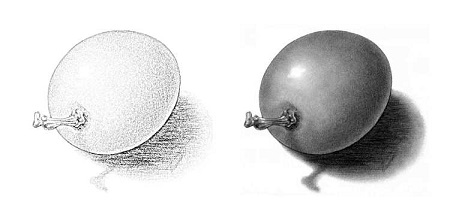
\includegraphics{imagens/luz-e-sombra-para-produzir-volume.jpg}

	\cite{Grafitti_2019}
\end{figure}


Como podemos observar que na figura acima, a imagem da esquerda apresenta apenas um rascunho, sem uso das técnicas de iluminação a portanto a noção de volume e profundidade não fica muito claro, por outro lado a imagem da direita sendo algo mais agradável nas pinturas como é possível notar, além do mais várias composições de cores da luz retratada em uma imagem pode trazer vislumbres fantásticos.

Com a chegada dos primeiros modelos em três dimensões, como cubos, piramides e esferas entre outros, foi possível enxergar através de uma tela, um objeto qualquer que fosse e isso mudou tudo, hoje podemos ver vários exemplos de modelos que está em nossa realidade, como a impressora 3D ou o \textit{Billboard}\footnote{apresentado em Tóquio, uma televisão imensa que pode captar imagens como se fossem 3D, criando um aspecto de profundidade pela sua curvatura}, pois é com ela que foi possível ver a grande beleza dos modelos, é por esse motivo pelo qual atualmente a iluminação é essência para nos causar a sensação de volume, sem pensar nos algoritmos mais robustos como \textit{ray tracing} que segundo \citeonline{shirley_2008} retrata, é um algoritmo onde através de uma janela, os raios são direcionados para as imagens. As superfícies são perdidas ou atingidas por cada pixel, que é representado por um raio. Ao atingir uma superfície, o raio se refrata e continua em um novo curso, causando a formação de luzes adicionais nos arredores.

Porém para os artistas chegarem perto dos algoritmos de iluminação que criam visuais impecáveis em três dimensões, as pinturas e artes foram obrigadas a criar um volume e melhorar a iluminação, pois como a luz funcionava de forma sistemática em três dimensões, as artes puderam abrir espaço em uma variação de cores e paletas diferenciadas que trazem um dinamismo maior.

Por isso atualmente a iluminação se tornou algo tão importante para o mundo, que não importa mas o estilo que é usado, é uma parte essencial. É nesse momento em que chegamos ao cerne do problema, pois com essa importância que a iluminação tem sobre a arte e os avanços tecnológicos cada vez mais ligados a ter um \textit{design} rápido e com eficiência, ferramentas que criam a luz em pinturas, desenhos, objetos, \textit{sprites} ou até logos poderia impactar a arte de maneira eficiente e até mesmo para aumentar a comunidade, fazendo com que várias pessoas iniciantes que não conseguem bons resultados possam aparecer no mundo do \textit{design}.

\section{Objetivos}

\subsection{Objetivo Geral}
O objetivo do trabalho é simular a iluminação em imagens digitais de média e baixa resolução por meio do desenvolvimento de uma ferramenta.

%O objetivo do trabalho é criar uma ferramenta que possa, a partir de uma imagem qualquer, gerar um ambiente tridimensional que irá simular a iluminação de forma natural.

\subsection{Objetivos Específicos}
\begin{itemize}
	\item Encontrar algoritmos que têm o propósito de iluminar cenas bidimensionais;
	\item Criar um protótipo e desenvolver a ferramenta para iluminação;
	\item Realizar testes na ferramenta Relight que será analisado para comparação dos resultados.
\end{itemize}
	\chapter{Revisão da Literatura}
\label{cap:02}

A segmentação de imagem, fundamentada em conceitos matemáticos, antecede o desenvolvimento das inteligências artificiais modernas e oferece uma vasta gama de métodos que exploram a relação entre \textit{pixels} adjacentes para identificar similaridades e descontinuidades na imagem. Segundo \citeauthorandyear{7359305} e \citeauthorandyear{ZAITOUN2015797}, essas técnicas se dividem principalmente em segmentações baseadas em camadas e em blocos, cada uma com abordagens e subcategorias específicas, como a detecção de bordas e a análise de profundidade e aparência dos objetos.

Já segundo \citeauthorandyear{electronics12051199}, os métodos de segmentação de imagens podem ser organizados em três categorias principais: segmentação clássica, co-segmentação e segmentação semântica baseada em \textit{Deep Learning}. Cada uma dessas categorias aborda a segmentação com diferentes técnicas e algoritmos, cada qual voltado para necessidades específicas de processamento e aplicação. A figura \ref{fig:segmentacao} mostra esses diferentes métodos de segmentação, organizando-os em categorias principais e destacando os principais algoritmos em cada abordagem.

\FloatBarrier
\begin{figure}[ht]
    \caption{Diagrama criado por \citeauthorandyear{electronics12051199}}
    \centering
    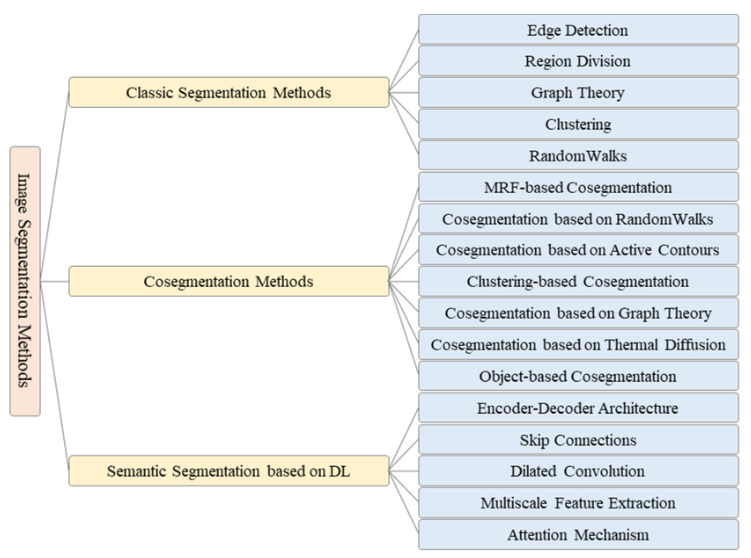
\includegraphics[scale=0.5]{imagens/metodos_segmentacao.png}
    \label{fig:segmentacao}
\end{figure}
\FloatBarrier

\section{Segmentação Baseada em Camadas}

No documento feito por \citeauthorandyear{electronics12051199} A \textbf{segmentação clássica} inclui técnicas que se concentram em características locais da imagem, como bordas e regiões como citado pelos outros autores também, mas ele aborda alguns conceitos diferentes como a \textbf{co-segmentação}, que foca na extração de objetos comuns em múltiplas imagens, considerando informações de contexto para identificar objetos similares. Por fim, a \textbf{segmentação semântica com \textit{Deep Learning}} incorpora redes neurais profundas que identificam objetos com precisão ao aprender características complexas diretamente de grandes conjuntos de dados anotados.

A segmentação baseada em camadas, conforme proposta por \citeauthorandyear{6042883}, é uma abordagem que organiza objetos em uma hierarquia de camadas, onde cada camada representa um objeto ou uma parte de objeto na imagem. Essa técnica permite que objetos sejam compostos e organizados em uma estrutura que leva em consideração tanto a aparência quanto a profundidade relativa de cada objeto na cena.

O método de \citeauthorandyear{6042883} utiliza máscaras de forma derivadas de detectores de objetos, as quais são compostas em camadas para criar uma segmentação que engloba tanto rótulos de classe quanto rótulos de instância. Com isso, a abordagem considera a organização espacial e relacional dos objetos, permitindo a detecção de elementos mesmo quando oclusos ou parcialmente visíveis, ao inferir o layout da cena com base em uma distribuição probabilística das camadas.

Cada camada é ordenada em profundidade, atribuindo objetos com maior pontuação em primeiro plano e outros objetos em segundo plano. Essa estruturação permite que o sistema identifique transições e relacionamentos entre diferentes camadas, ajudando a criar segmentações precisas, principalmente em cenários complexos onde múltiplas instâncias de objetos podem se sobrepor ou interagir de forma dinâmica. A partir dessa hierarquia, o modelo é capaz de reconciliar informações de alto nível com detalhes de baixo nível, integrando informações de cor e textura com os contornos e formatos dos objetos segmentados.

A segmentação em camadas não só melhora a precisão da rotulação de pixels, mas também possibilita uma compreensão mais profunda das interações entre objetos. Essa característica é particularmente vantajosa para a segmentação de imagens que contêm múltiplas instâncias e classes, onde a separação de camadas facilita a correta identificação de fronteiras e a resolução de ambiguidades visuais.

\section{Segmentação baseada em blocos}

Já os métodos de Segmentação de Imagem Baseados em Blocos, segundo \citeauthorandyear{ZAITOUN2015797}, podem ser categorizados em duas propriedades principais: descontinuidade e similaridade. Essas técnicas de segmentação dividem-se em várias abordagens, incluindo aquelas que se concentram em características como cor, continuidade, similaridade e bordas, permitindo a criação de subcategorias específicas de acordo com o processo de divisão aplicado.

Entre as abordagens principais, destacam-se os métodos baseados em bordas abordado por \citeauthorandyear{Mayangky_Merlina_Prasetyo_Amelia_Irsictia_Putri_2024}, que se concentram em detectar descontinuidades na intensidade da imagem para identificar transições abruptas entre diferentes objetos ou regiões. Alguns dos métodos clássicos de detecção de bordas incluem a \textbf{Detecção de Bordas de Roberts}, que utiliza operadores cruzados para calcular o gradiente espacial e é amplamente valorizada pela simplicidade e eficiência, sendo ideal para aplicações que exigem baixo custo computacional; a \textbf{Detecção de Bordas de Prewitt}, que calcula a magnitude e orientação das bordas usando uma máscara de convolução 3x3, tornando-se mais robusta do que o método de Roberts, embora ainda suscetível a ruídos; e a \textbf{Detecção de Bordas de Sobel}, que aplica uma máscara 3x3 rotacionada em 90º para suavizar ruídos enquanto calcula o gradiente das bordas, sendo amplamente utilizada devido à sua eficácia na detecção de bordas.

Com os avanços na inteligência artificial e nas técnicas de computação evolutiva, surgiram métodos de detecção de bordas mais sofisticados. Entre eles, o método \textbf{Baseado em Lógica Fuzzy} que é descrito por \citeauthorandyear{info8030104} como uma lógica que utiliza conjuntos fuzzy que permitem que cada pixel pertença a múltiplas regiões, oferecendo flexibilidade em imagens com transições suaves. Já o método \textbf{Baseado em Algoritmos Genéticos} inspira-se na teoria da evolução, utilizando processos de seleção, cruzamento e mutação para identificar as bordas de maneira eficiente, sendo particularmente útil em padrões complexos. O método \textbf{Baseado em Redes Neurais}, por sua vez, utiliza redes neurais artificiais treinadas para aprender padrões de bordas ajustando os pesos entre suas camadas, sendo altamente eficaz na detecção de bordas em cenários com variabilidade de padrões. 

A integração do big data com o avanço dos hardwares modernos permitiu que a inteligência artificial atingisse novos patamares de desempenho na segmentação de imagens. A habilidade de processar grandes volumes de dados possibilita que a IA identifique padrões e características em imagens de maneira rápida e precisa. Segundo \citeauthorandyear{carvalho_2021}, o uso de \textit{deep learning} e de técnicas de machine learning aprimora ainda mais essa precisão, tornando a segmentação detalhada e eficiente, essencial para diversas aplicações inovadoras.

\section{Segment Anything}

Inserido nesse contexto e com base no artigo criado por \cite{kirillov2023segany} o modelo Segment Anything (SAM) é um novo avanço na área de segmentação de imagens, proporcionando uma abordagem generalista que visa resolver diversos problemas de segmentação utilizando diferentes tipos de dados e prompts. Com um conjunto de dados extenso e uma arquitetura inovadora, o SAM permite a criação de máscaras de segmentação em tempo real e com capacidade de generalização para novos conjuntos de dados.

\subsection{Motivação e Contexto}

A segmentação de imagens tem sido revolucionada pelo surgimento de métodos de \textit{deep learning}, como o Segment Anything Model (SAM), que permite uma segmentação versátil e de alta escala. A segmentação de imagem visa identificar e isolar regiões ou objetos dentro de uma imagem, o que é essencial em várias aplicações de visão computacional. Métodos convencionais, entretanto, exigiam grande quantidade de dados rotulados e intensa supervisão manual. O SAM introduziu uma abordagem de zero-shot, possibilitando segmentações precisas em novos conjuntos de dados sem a necessidade de re-treinamento, utilizando prompts como caixas delimitadoras e pontos para indicar regiões de interesse \cite{ke2023segmenthighquality}.

Apesar de seu impacto, o SAM apresenta limitações ao lidar com bordas complexas e objetos finos. Para superar essas limitações, o HQ-SAM foi proposto como uma extensão de alta qualidade do SAM, incorporando um token de saída especializado e técnicas de fusão de características globais e locais para melhorar a definição das bordas e a precisão da segmentação em objetos detalhados e sobrepostos. Esses avanços garantem que o HQ-SAM preserve a flexibilidade e a generalização zero-shot do SAM original enquanto aumenta significativamente a acurácia da segmentação \cite{ke2023segmenthighquality}.

\subsection{Arquitetura do SAM}

A arquitetura do SAM é composta por três principais componentes: um codificador de imagens, um codificador de prompts e um decodificador de máscaras. O codificador de imagens gera um embedding (representação) da imagem que pode ser reutilizado para diferentes prompts. O codificador de prompts permite que o SAM aceite uma variedade de entradas, como pontos, caixas delimitadoras, e até mesmo textos para identificar as áreas de interesse na imagem. O decodificador de
máscaras, então, gera as máscaras de segmentação apropriadas a partir dessas entradas. O SAM é projetado para ser eficiente, processando prompts em tempo real.

\subsection{Conjunto de Dados SA-1B}

Para treinar o SAM, foi desenvolvido o conjunto de dados SA-1B, que contém mais de 1 bilhão de máscaras de segmentação provenientes de 11 milhões de imagens. Essas imagens são diversas, de alta resolução, e foram obtidas respeitando
questões de privacidade. Esse conjunto de dados é, até o momento, o maior já construído para a tarefa de segmentação, superando os bancos de dados existentes em termos de diversidade e volume. O SAM é capaz de gerar máscaras de
segmentação automaticamente a partir dessas imagens, tornando-se uma ferramenta poderosa para a criação de novos conjuntos de dados e modelos de visão computacional.

\subsection{Aplicações e Resultados}

O Segment Anything Model (SAM) foi amplamente testado em tarefas de segmentação, como a segmentação de objetos a partir de pontos, detecção de bordas e segmentação de objetos sobrepostos, demonstrando forte desempenho e flexibilidade. Em cenários complexos, o SANeRF-HQ aprimora o SAM para segmentação em 3D de alta qualidade, utilizando prompts e campos de densidade para garantir consistência entre múltiplas visualizações. Os resultados mostram uma melhoria significativa em relação aos métodos anteriores, mantendo generalização zero-shot e alta acurácia ao longo de diferentes conjuntos de dados \cite{liu2024sanerfhqsegmentnerfhigh}.

\subsection{Comparações com Métodos Tradicionais}

O SAM apresenta várias vantagens em relação a métodos tradicionais de segmentação, como o Crescimento de Regiões. Enquanto os métodos tradicionais exigem parâmetros e pré-processamento mais específicos para funcionar corretamente, o SAM, por meio de sua arquitetura flexível e escalável, permite segmentação em uma ampla gama de imagens com menos intervenção manual. Além
disso, sua capacidade de processar múltiplas máscaras para um único prompt o torna eficaz para cenários onde a ambiguidade está presente, como a detecção de partes de objetos sobrepostos.

\section{Trabalhos Correlatos}

Nesta seção são apresentados os trabalhos correlatos ao proposto neste trabalho

\subsection{Segmentation by grouping junctions}

A segmentação de imagens tem evoluído significativamente com a introdução de métodos baseados em aprendizado profundo.\citeauthorandyear{minaee2020imagesegmentationusingdeep} realizam uma extensa revisão sobre métodos de segmentação com redes neurais, destacando abordagens como redes totalmente convolucionais (FCN), arquiteturas encoder-decoder e redes piramidais de múltiplas escalas, que são amplamente adotadas. Estes métodos permitiram avanços consideráveis na precisão e na generalização dos modelos, especialmente para aplicações em imagens médicas e na análise de cenas complexas, onde a precisão é crucial.

\subsection{Monocular depth estimation based on deep learning: An overview}

A estimação de profundidade monocular é um problema fundamental em visão computacional. Métodos baseados em aprendizado profundo (deep learning) têm sido estudados e alcançaram resultados promissores. Existem três categorias de métodos: supervisionados, não supervisionados e semi-supervisionados. Arquiteturas de rede neural como CNNs, RNNs e GANs são utilizadas. O artigo de \cite{zhao2020monocular} apresenta uma visão geral desses métodos e discute desafios e oportunidades.
	\chapter{Metodologia}
\label{cap:03}

Descrever metodologia, materiais e métodos utilizados no estudo, bem como os procedimentos experimentais realizados, nesta etapa será descrito vários assuntos sobre os passos a serem realizados iniciando com o levantamento dos dados, para uma analise e estudo posteriormente analisando todos os processos que são realizados, afim de iniciar o desenvolvimento.


\begin{figure}[ht]
\caption{Passos feito na plataforma miro}
\centering
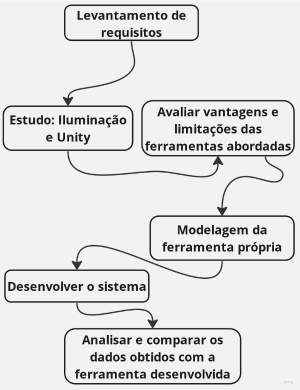
\includegraphics{imagens/Diagrama.jpg}

Fonte: Feito pelo autor
\label{fig:diagrama}
\end{figure}

\section{Levantamento de Requisitos}

Nessa sessão será abordado a pesquisa qualitativa feita a partir da ferramenta \textit{Relight} que usa de um algoritmo para identificação de camadas em uma imagem, assim, quando a imagem é colocada na ferramenta ela faz um mapeamento das áreas altas e baixas para criar as camadas, por esse motivo as camadas que são denominadas como mais alta recebe mais luz do que as mais baixas.

Porém a ferramenta tem uma funcionalidade a mais onde é possivel definir em que nível está a luz, fazendo com que a iluminação do objeto possa vir das camadas mais a baixo para as camadas acima, está ferramenta com a luz funciona como um pincel de adicionar em softwares de pintura, pois ela recebe a luz já existente na foto e complementa por cima com a luz própria, podendo ser de qualquer cor.

A seguir será mostrado na tabela, onde terá a avaliação qualitativa referente a vários tipos de imagens testadas a partir da ferramenta, que para efeitos deste trabalho serão utilizados os valores de alta resolução como acima de 720 pixels, média resolução entre 720 e 256 pixels e baixa resolução abaixo de 256 pixels, retratado na tabela:

Avaliação qualitativa da ferramenta

\begin{tabular}{l r r r}
Imagem & Alta Resolução & Média Resolução & Baixa Resolução\\
Objetos & Funciona  & Funciona  & Restrição\\
Humanos & Funciona  & Funciona  & Restrição\\
Paisagens & Funciona & Problema &  Problema\\
\end{tabular}

Nessa tabela, foi adotado três categorias para descrever o funcionamento: Funciona, Restrição e Problema.
A primeira categoria é utilizada para descrever que a imagem utiliza se comportou de forma correta, Restrição é a categorização para as imagens que funcionam mas em alguns casos ou áreas da imagem geram problemas, já a categoria Problema indica os casos onde a luz não reconhecia as formas de maneira correta.

\section{Estudo: Iluminação e Unity}
Nesse estudo será demonstrado algumas das partes que serão necessárias para o desenvolvimento da ferramenta, como a seguir que se iniciará com a iluminação nas histórias em quadrinhos.
Sempre que vemos uma cor clara e logo depois uma escura, isso significa que há um relevo muito grande ali, por exemplo  na Figura \ref{fig:batman}

\begin{figure}[ht]
\caption{História em quadrinhos, Batman}
\centering
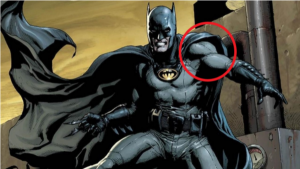
\includegraphics{imagens/batman.png}

Fonte: \cite{Bazela2022-yg}
\label{fig:batman}
\end{figure}    

Nesse quadrinho do Batman, podemos ver que em seu ombro está muito claro e logo acima onde sua capa está vem uma cor muito escura, isso nos mostra que a profundidade da capa é grande, ao ponto de não chegar nenhuma luz até ela, é claro que precisamos levar em consideração que nas HQ’s em geral os contrastes são muito maiores, porque traz esse volume nos trajes.

Partindo para o ramo da \textit{Unity} será preciso um aprendizado todo relacionado a iluminação dentro da ferramenta, uso dos objetos em cena e manipulação deles, pois para o desenvolvimento será necessário a criação de uma malha que forme a imagem, um sistema de camadas para que possa estabelecer profundidade, um sistema de alteração e manipulação da posição, cor e luminosidade do ponto de luz. E por fim um estudo básico de toda interface da \textit{Unity}.

Outro ponto importante no estudo, será a linguagem de programação \texttt{C\#} que é usada como alicerce para qualquer código que precise ser estruturado lá dentro, desde instanciar objetos dentro da cena até modificar configurações de câmera como movimento, posicionamento e angulo até para recebimento dos arquivos

\section{Avaliar vantagens e limitações das ferramentas abordadas}

O \textit{Relight} é uma ferramenta muito boa para processos de iluminação tanto para cenários como personagens, com uma boa modificação como profundidade, posição, cor e luminosidade, dando para o usuário a liberdade de dar personalidade as suas imagens.

Mas ainda existe várias limitações e elas que serão retratadas nessa seção, como foi visto na analise a cima na tabela é possível notar que quanto menor a imagem é, menos funcional ela passa a ser, por exemplo imagens em baixa resolução ou pixeladas começam a ter muitos problemas pois a luz não consegue distinguir os objetos na cena e muito menos paisagens pois com tantas cores perto uma das outras transforma a cena em uma desordem visual.

\section{Modelagem da ferramenta}

Uma malha deverá ser criada por cima de toda a imagem e definir um inteiro para a profundidade, cada \textit{pixel} dá imagem deve receber uma profundidade como pode se observar na Figura \ref{fig:sketch}

\FloatBarrier
\begin{figure}[ht]
\caption{Rascunho elaborado pelo autor}
\centering
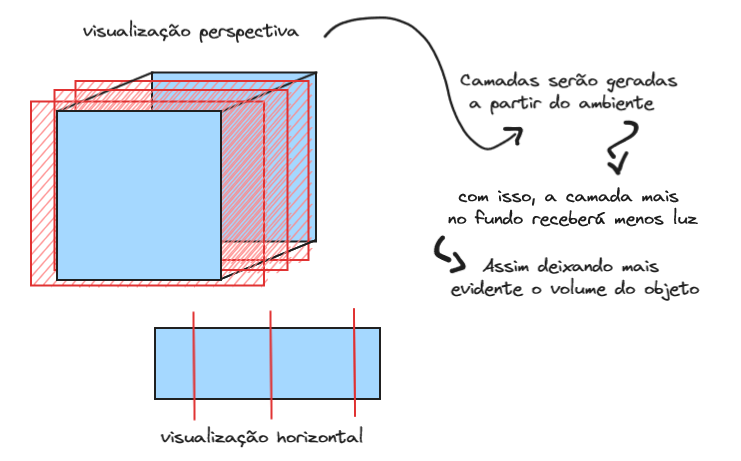
\includegraphics[scale=0.5]{imagens/Sketch.png}

\label{fig:sketch}
\end{figure}    
\FloatBarrier

Assim ele vai numerar toda a malha de \textit{pixels} na tela com números que podem ter uma variação maior dependendo do tamanho da imagem ( no caso de exemplo)

Será calculado de 1 a 9, mas com imagens imensas em alta resolução podemos pensar em usar de 1 a 100 ou até mais

Podemos pensar que dessa forma será possível utilizar essa profundidade para produzir uma luz pelas laterais ou pela frente e até atrás de elementos, sem perder sua funcionalidade até mesmo em imagens pequenas

Além disso, cada um desses valores definidos em cada \textit{pixel} da imagem, vão servir de referencia para criação de vários objetos, ele levará em consideração a distância e a variação de cor que foi atingida

Como por exemplo, se existir um objeto a frente da camada 1 até a 10 e um objeto atrás que está na camada 15, essa distancia de 5 camadas irá fazer o objeto dá frente se separar com o de trás transformando a cena com dois objetos ao invés de um


\section{Justificativa das Tecnologias a serem adotadas}

Será utilizado a IDE Visual Studio para a criação dos códigos que serão importados na \textit{Unity}, foi optado ele pois é o sistema mais robusto para a utilização do \texttt{C\#}.

Para o processo de desenvolvimento efetivo, além da IDE será usado a \textit{game engine}, Unity, que foi escolhida pela simplicidade em aplicar luz e criação de objetos bidimensionais em ambientes Tridimensionais, ou como é conhecido 2.5D, para assim poder criar com efetividade a malha e a luz aplicada a ela

\section{Avaliação Qualitativa}

Logo após todo o processo estiver concluído, chega a etapa da avaliação, nesse tópico irá apresentar como será feita a avaliação dos resultados obtidos a partir das analises feitas anteriormente, nesta comparação será possível avaliar os seguintes pontos, primeiramente a alteração em imagens de baixa resolução se é possível a partir desse novo algoritmo e se as vantagens irão se permanecer. Outro ponto que poderá ser analisado será a eficacia de executar a ferramenta e se ela é possível a partir dos cálculos necessários.
	\chapter{Análise dos Resultados}
\label{cap:04}
Neste capítulo, são apresentados e discutidos os resultados obtidos na aplicação dos métodos de segmentação de imagens propostos neste trabalho, com ênfase nas imagens de média e baixa resolução. Utilizando o modelo Segment Anything (SAM), avaliou-se a eficácia do método utilizado, que utilize inteligencia artificial para aprimorar a precisão da segmentação.

Para uma análise quantitativa robusta, foram adotadas as métricas Mean Squared Error (MSE) e Normalized Cross-Correlation (NCC), além de um método específico criado para complementar a avaliação dos segmentos. Estes indicadores foram aplicados para avaliar a qualidade das segmentações produzidas, comparando-as com padrões de segmentação existentes. Este capítulo tem, portanto, como objetivo apresentar as análises qualitativas e quantitativas dos resultados, destacando os avanços e as limitações do método proposto em relação aos métodos tradicionais.

\section{Agilidade e Eficiência}
Nessa seção será abordado o fator velocidade para o processo ser finalizado, ou seja, independente dos resultados qual a margem de tempo destinada apenas a realização da segmentação das imagens, lembrando que isso seria apenas um fragmento de todo o desenvolvimento da ferramenta.

Como o esperado, foi identificado nos computadores usados para executar o código uma quantidade de tempo razoável até sua finalização,apesar disso, entre eles houveram minímas diferenças de tempo de execução, mesmo com abruptas diferenças de processamento, em seguida será mostrado as propriedades de cada um deles, para uma melhor comparação da média dos resultados obtidos em termos de desempenho, como mostra a \ref{tab:comparacao_desempenho}.

\begin{table}[h!]
	\centering
	\begin{tabular}{|p{4cm}|p{5cm}|p{5cm}|}
	\hline
	\textbf{Propriedade}         & \textbf{Computador}                & \textbf{Notebook}                     \\ \hline
	\textbf{Processador}          & AMD Ryzen 5 1400 Quad-Core        & Intel Core i5-1235U                   \\ \hline
	\textbf{Número de Threads}    & 8                                 & 12                                    \\ \hline
	\textbf{Frequência Base}      & 99.8 MHz                          & 99.8 MHz                              \\ \hline
	\textbf{Frequência Máxima}    & 3192.4 MHz                        & 3790.7 MHz                            \\ \hline
	\textbf{Memória RAM}          & 16 GB DDR4                        & 8 GB DDR4                             \\ \hline
	\textbf{Frequência da Memória}& Não especificada                  & 1596.1 MHz                            \\ \hline
	\textbf{\textit{Chipset}}     & AMD B350                          & Intel Alder Lake rev. 04              \\ \hline
	\textbf{Placa Mãe}            & Asus Prime A320M-K/BR             & Modelo LNVNB161216                    \\ \hline
	\textbf{\footnote{VRAM}}      & 4 GB NVIDIA 1050 TI               & Intel UHD Graphics                    \\ \hline
	\end{tabular}
	\caption{Comparação de Desempenho entre Computador e Notebook}
	\label{tab:comparacao_desempenho}
\end{table}

Com a tabela é possível notar que apesar da comparação semelhante quando nos referimos ao processamento das maquinas, é extremamente necessário levar em consideração o uso da placa gráfica para o processamento com o suporte do CUDA, que nada mais é do que um sistema criado pela NVIDIA a fim de utilizar as placas gráficas como potencializadores para integração de inteligências artificiais, contudo, os resultados em termos de velocidade de execução foram muito próximos como é possível notar no gráfico \ref{fig:grafico_desempenho}

\FloatBarrier
\begin{figure}[ht]
    \caption{Análise de desempenho}
    \centering
    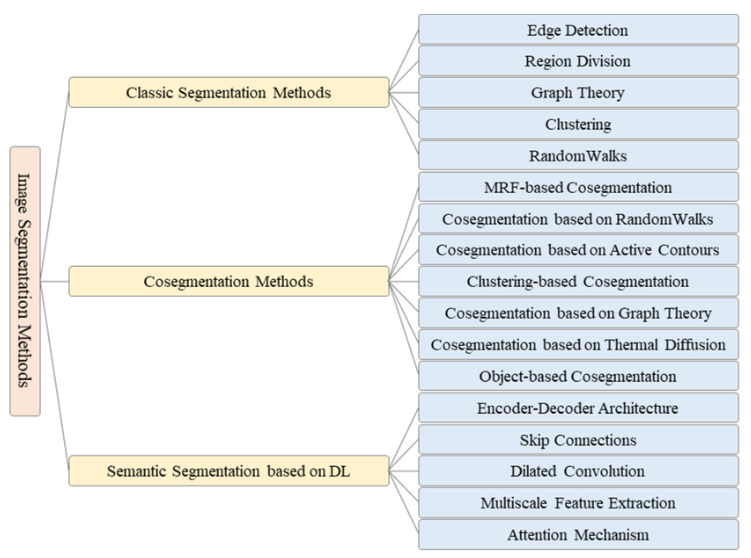
\includegraphics[scale=0.5]{imagens/metodos_segmentacao.png}
    \label{fig:grafico_desempenho}
\end{figure}
\FloatBarrier


\section{Resultados/Impactos}

Resultados.

\section{Cronograma do Trabalho}

Segue abaixo o cronograma de trabalho das atividades realizadas até a Avaliação Final de TCC.

\begin{enumerate}
	\item Elaboração da Introdução
	\item Elaboração da Revisão da Literatura
	\item Elaboração da Metodologia
	\item Estudo sobre a \textit{Unity} e Iluminação
	\item Desenvolvimento da ferramenta
    \item Alteração do escopo em decorrência das dificuldades técnicas 
    \item Geração das imagens para análise
    \item Análise e elaboração das métricas
    \item Desenvolvimento dos capítulos
    \item Revisão e Conclusão
\end{enumerate}

\FloatBarrier
\begin{figure*}[!htbp]
	\centering
	\includegraphics[scale=0.8]{imagens/Cronograma.png}
\end{figure*}
\FloatBarrier



	\chapter{Conclusões Parciais}
\label{cap:05}

Foi descrita a modelagem da ferramenta própria, que envolve a criação de uma malha por cima da imagem para definir a profundidade e a variação de cor, permitindo a manipulação da luz. Além disso, foi citado as tecnologias adotadas, como o Visual Studio para programação em \textit{C\#} e a Unity como a game \textit{engine} escolhida.

Para avaliar a eficácia da ferramenta, foi planejado realizar uma avaliação qualitativa dos resultados obtidos, incluindo a análise da alteração de imagens, a viabilidade da ferramenta e a eficácia dos cálculos realizados. Para fim é esperado que a ferramenta esteja concluída mesmo que de forma manual, para que ocasionalmente possa ter um progresso posterior em outros trabalhos.


%São descritas claramente as conclusões retiradas das discussões e dos experimentos realizados no decorrer da pesquisa, e finalizada a parte textual do trabalho. Recomendações são declarações concisas de ações, julgadas necessárias a partir das conclusões obtidas, a serem usadas no futuro. Ou seja, lembre-se de apresentar os possíveis trabalhos futuros derivados do seu trabalho.
	
	
	% ----------------------------------------------------------
	% Referências bibliográficas
	% ----------------------------------------------------------
	\postextual
	\bibliography{referencias}
	
\end{document}
